\chapter{3D Modeling of the breast}\label{chap:modeling}

\section*{}

In order to achieve a prediction of the aesthetic outcome after a BCS the best option is to describe the breast using 3D models. Some models can be reached with several techniques, but all of them retrieve a model with some compression or mechanical force present.

Due to the importance on medical imaging to find a smooth surface that fits a set of 3D unstructured data to describe and represent anatomical structures, many alternatives have been found over the years. Being a complicated problem and due to the variability and difference between the shape of human breasts, a lack of work on this field was led to \cite{De2016}.

The present chapter starts by presenting several data acquisition techniques, in section \ref{sec:acquisition}, that could provide the information for generating 3D models. The data may be represented using for example parametric and deformable models presented in section \ref{sec:param} and section \ref{sec:deform}, respectively. At the end of the chapter some existing frameworks used for breast augmentation and plastic surgery are referred in section \ref{sec:ferramentas}, such as the methods that they use in order to acquire and model 3D data.


\section{Data Acquisition}\label{sec:acquisition}

Despite of all the several ways to describe and represent the shape of breast, the 3D imaging yields more information than multiple conventional photographs. Given this, 3D models are the best and more realistic way to evaluate the shape and size of the breast, its symmetry, contour, volume and surface area \cite{Kim2008}.

Multiple attempts have been done to represent breast as a 3D object. Those attempts have started by using Magnetic Resonance Imaging (MRI), Computed Tomography (CT) and 3D surface imaging systems. Bücking et al. in \citep{3dprintplos} describes the use of CT and MRI data to generate 3D models of anatomical human parts in order to 3D print the obtained models. In this case a pre-processing of the data was done considering two main steps: image segmentation, where the image was labelled and partitioned into several areas and regions ignoring the noisy regions of the image; and a mesh refinement, repairing and smoothing the models' discontinuities. The authors also mentioned that CT was used instead, when segmenting structures with low or high densities. MRI are best used in soft tissues due the high contrast on this cases.

An alternative to retrieve 3D models of the patient's torso was proposed in \cite{Costa2014}. This approach used a low-cost depth sensor (Microsoft Kinect) to acquire several views of patient's torso in order to perform a point cloud registration of the breast. The point cloud registration process is subdivided into two parts: coarse registration and fine registration. In order to generate the point cloud that would serve as input in the coarse registration, the raw RGB-D data acquired by the sensor were pre-processed. The pre-processing started by segmenting and then filtering the depth image in order to remove the noise on the edge and silhouette of the object. Given the retrieve point could, a Tessellation-based coarse registration uses depth data to align the point clouds. The alignment was done by a pose estimation, to reduce the initial misalignments; a keypoint selection to identify some correspondences between different point clouds; and a correspondence estimation and validation to find the better coarse alignment.

According to \citet{apenn}, the acquisition of MRI data consist of several MRI axial slices of the breast and ensures the 3D visualization of the patient's breast. In the cases where the acquisition of MR images is not axial, it can be converted posteriorly. Thereafter and despite of the semi-automatic segmention of the MRI data contours, the images required a manual segmentation in order to differ parenchyma, fat and lesion tissues. Based on the segmentation results and the defined contours it is possible to calculate a few reference points and then generate a 3D computational mesh. The generated mesh is represented by parallel planes limiting the breast's contour.

\section{Parametric Models}\label{sec:param}

Once the raw 3D data are obtained and due to the need to easily manipulate it, depending on its application, the information acquired may need to be represented or transformed in any other type of 3D representation. In the case of medical application such as representing human organs, the parametric models are widely used. An application of parametric models was described in \cite{Vision1998} when representing the left ventricle of the heart. These models have as advantage using superquadrics parameters allowing to represent objects with rounded edges or corners that may resemble a wide variety of human organs. 

The fitting of superquadrics to 3D unstructured data being a problem, it was already investigated, what led to some robust and fast methods that solved it. A superquadric refers to different sets of superellipsoids, supertoroids or even one or two pieces of superhyperboloids. And despite of the general use of superellipsoids, presented in Figure \ref{fig:superellipsoids} the other objects can also be used in order to describe different shapes.

\begin{figure}[H]
\begin{center}
    \leavevmode
    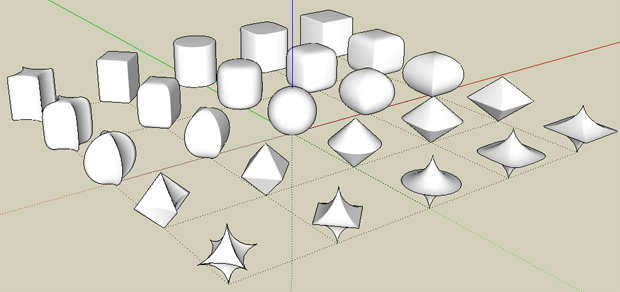
\includegraphics[width=0.85\textwidth]{superellipsoid}
    \caption[Examples of superellipsoids]{Examples of superellipsoids \protect\footnotemark}
    \label{fig:superellipsoids}
  \end{center}
\end{figure}
\footnotetext{\url{http://regular-polygon.com/plugins/superellipsoid/}}

A superquadric is obtained by the spherical product of two 2D curves. In the case of a superellipsoid, it is described by the following equations.

\begin{equation}
\left ( \left ( \left ( \frac{x}{a_1} \right )^{\frac{2}{\varepsilon_2}} + \left ( \frac{y}{a_2} \right )^\frac{2}{\varepsilon_2} \right )^\frac{\varepsilon_2}{\varepsilon_1} + \left ( \frac{z}{a_3} \right ) ^\frac{2}{\varepsilon_1} \right ) ^ \frac{\varepsilon_1}{2} = 1
\end{equation}

The parameters $a_1$, $a_2$ and $a_3$ are scaling factors corresponding to the coordinate axis, and $\epsilon_1$ and $\epsilon_2$ represent the squareness of the original superellipsoids.

A smaller $\epsilon$ represents a superellipsoid similar to a square, $\epsilon$ equal to 1 represents a circle and $\epsilon$ equal to 2, a shape with a flat bevel and a superellipsoid with larger $\epsilon$ defines a pinched shape.

In order to pose the superquadric on an axis system, 6 more parameters are required.

\begin{equation}
Xw=T.Xs, T= 
\begin{bmatrix}
R&t\\
0&1\\
\end{bmatrix}
\end{equation}

R is a 3x3 matrix and t a 3x1 matrix representing the rotation and translation, in relation to the referrals' origin, of the superquadric respectively.

As soon as the most adequate superquadric is chosen, it must fit the 3D data that we want to represent. Despite of the good global approximation of a shape, superquadrics are too limited when representing more complicated surfaces. This problem usually occurs due to the symmetry of the superquadrics. A possibility to overcome is the utilize deformable models presented on section \ref{sec:deform} or its application of the parametric models refereed in \cite{Pernes2014}.



\section{Deformable Models}\label{sec:deform}
Representing the 3D data of the patient's breast using Deformable models will allow generating and manipulating complicated curves and surfaces. The deformations that would be applied in order to generate that kind of complex data can be categorized in two different methods Physical Methods and Non-Physical Methods. While the Non-Physical Methods manually manipulate and deform the objects by adjusting one or more parameters of the shape (that describe the more simple object), the Physical Method relies on the modification of the physical properties of the object through the application of external forces. In the case of Physical methods, the material's properties of the object also impact the deformation of the object \cite{Gibson97asurvey, De2016}.


\subsection{Non-Physical Models}

As mentioned before, the non-physical methods to deform object are done recurring to the alteration of model parameters. Widely used ways to represent curves defined by vectors of control point vary between Bezier curves, B-splines or non-uniform rational B-splines (NURBS).

The abovementioned approach in \cite{Pernes2014} and \cite{Vision1998} is based on the application of Free Form Deformation (FFD). The FFD allows to define the deformations by adjusting the space where the object lies and not by changing its control points. Another advantage of this approach is that the same deformation can be applied to the different models simultaneously.

On this specific approach the model is considered to be embedded in a box that can be changed in order to twist, bend or taper the model on its interior. Figure \ref{fig:FFD} shows the object embedded on the box of control points in \ref{fig:FFD_BB} and the result of the object deformation in \ref{fig:FFD_applied}. To accomplish this, the FFD formulation shall be done in the two following steps:

\begin{enumerate}
\item Compute the local coordinates of the object points in the frame defined by the box of control points.

\begin{equation}
X = X_{0} + s S + t T + u U,
\end{equation}

where \textit{s}, \textit{t} and \textit{u} are given by:

\begin{equation}
s = \frac{S. \left(X-X_{0} \right)}{S.S},   t = \frac{T. \left(X-X_{0} \right)}{T.T},   u = \frac{U. \left(X-X_{0} \right)}{U.U}, 
\end{equation}

\textit{X} represent each point of the objects by the coordinates (\textit{s},\textit{t},\textit{u}) and the box where the object is embedded is represented by the vertex \textit{$X_{0}$} and the box edges (\textit{S},\textit{T},\textit{U}).

The point \textit{X} is inside of the box if and only if \textit{s}, \textit{t} and \textit{u} have all values between 0 and 1.

The size of the embedding box is given by the parameters $a_{1}$, $a_{2}$ and $a_{3}$ of the superquadric and its rotation is given by the coefficients of the rigid transform $\varphi$, $\theta$, $\psi$, $t_{x}$, $t_{y}$ and $t_{z}$.

The volumetric grid of the box's control points $\left( l+1 \right)$ $\left( m+1 \right)$ $\left( n+1 \right)$ can be described by:

\begin{equation}
  \begin{cases}
  	x(\textbf{$P_{ijk}$}) = a_{1} \left(1-2 \frac{i}{l} \right) \\
  	y(\textbf{$P_{ijk}$}) = a_{2} \left(-1+2 \frac{j}{m} \right) \\
  	z(\textbf{$P_{ijk}$}) = a_{3} \left(1-2 \frac{k}{n} \right) 
  \end{cases}
\end{equation}

At last, the space alterations that the model will be put through may be represented as:

\begin{equation}
X = BP,
\end{equation}

where \textit{X} is a matrix NP x 3 (NP: number of control points = (l+1)(m+1)(n+1)) with the coordinates of the model points, \textit{B} is the deformation matrix ND x NP (ND: number of points on the object) and \textit{P} the NP x 3 matrix which contains coordinates of the control points $P_{ijk}$.

\item To achieve the best fitting of the model to the data we intent to represent, the displacement field must be reduced. This displacement refers to the distance between the model and the data points we will represent.

We are changing position of control points to fit X to the target model. Note that we are not fitting control points to sth.

As soon as the best fitting of the model is find, by changing the position of control points in order to make \textit{X} fit the target model, the position of point \textit{X} of the object may be computed.

\end{enumerate}

\begin{figure}[H]
\begin{tabular}{ll}
\subfloat[Box of control points with embedded object]{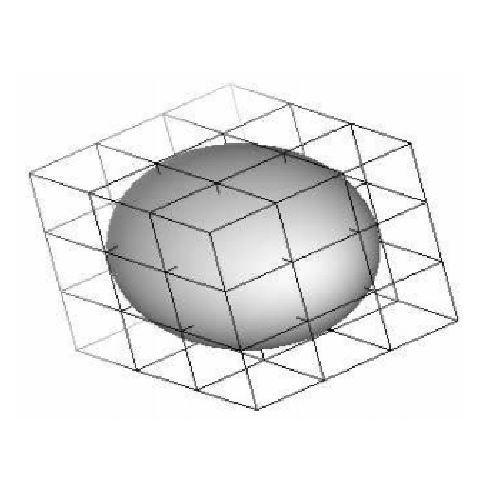
\includegraphics[width = 3in]{FFD_BB}\label{fig:FFD_BB}} &
\subfloat[Object of the deformed box]{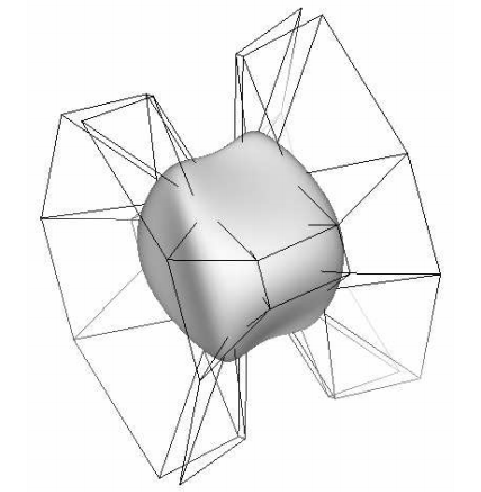
\includegraphics[width = 3in]{FFD_applied}\label{fig:FFD_applied}}
\end{tabular}
\caption[FFD deformation]{FFD deformation \cite{Vision1998}}
\label{fig:FFD}
\end{figure}

\subsection{Physical Models}
A well-studied physical model is mass-spring method which is used in modeling facial expressions. The proposed methodology described in \cite{Gibson97asurvey} uses three distinct layers of tissue in order to deliver a mesh of mass points corresponding to the dermis, a layer of fatty tissue and a layer of muscular tissue. The same approach has been adopted in the context of breast surgery \cite{1085f1d}, where a volumetric tetrahedral mesh representing the breast was computed from a semi-automatic segmentation procedure. Then the mesh was deformed based on the mass-spring model: the spring's rest length and stiffness were estimated and then applied to the uncompressed breast model in order to deform it to the real compressed one. Although being easy to construct and allow to deform the objects in more ways than other physical methods, mass-spring finds difficult to model incompressible volumetric objects or unbendable surfaces.

Another method with a great variety of applications is Finite Element Models (FEM). In contrast with the mass-spring method, FEM is more accurate, requiring a much larger computational power and being a very time consumption process. In a FEM, the object is divided into several elements joined by discrete node points. The desired deformation function is then applied to each element in order to find an approximation that satisfies an equilibrium expression relative to the intended deformation. The type of elements that are used to form the model are chosen according to the properties of the object, the trade-off between the computational power and the required accuracy. One of many examples of the application of FEM was described in \cite{Kurihara2004} where simullating the interacting between the soft tissue of a human hand and a deformable object. Considering the apllication of FEM in breast surgery, it has been used in \cite{Vavourakis2016}, whose proposed methodology will be further detailed.

\vspace{12mm}

Vavourakis et al. \cite{Vavourakis2016} proposed a surgical simulator based on a FEM. In order to simulate the wound healing effect described in \cite{Vavourakis2016} data was gathered though MRI as described in \cite{apenn}. The used mesh is constituted by two distinct types of isoparametric elements, shown on Figure \ref{fig:3d_mesh}:

\begin{itemize}
\item Solid 4-node trilinear isoparametric elements - used to represent the breast tissues except for the skin;
\item 3-node triangular isoparametric elements - used to represent the surface of the model: the breast's skin.
\end{itemize}

\begin{figure}[H]
\begin{center}
    \leavevmode
    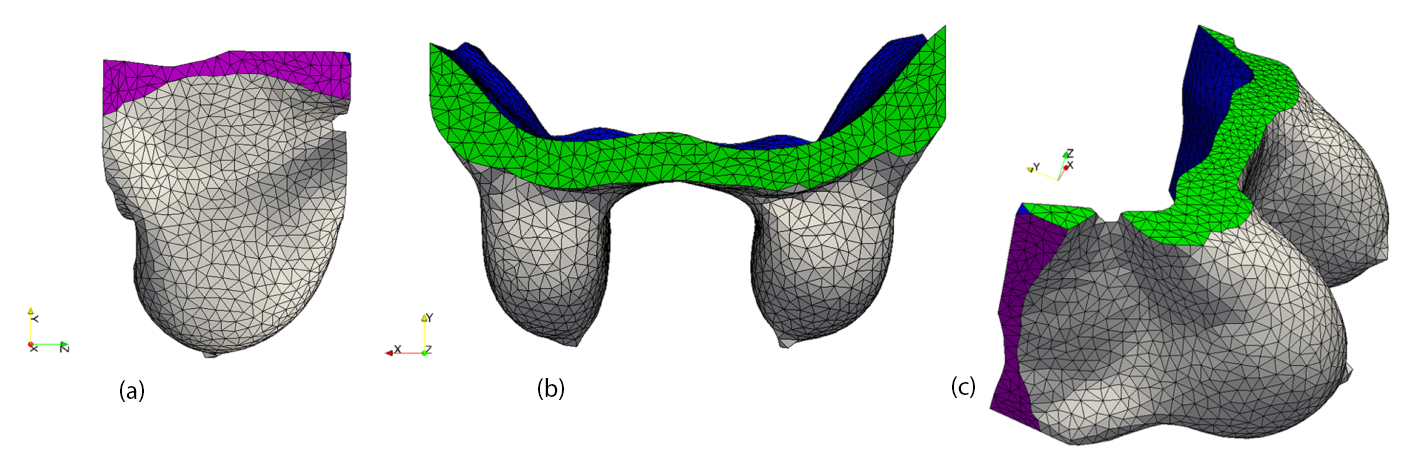
\includegraphics[width=0.85\textwidth]{FE}
    \caption[3D mesh with isoparametric elements]{\textbf{3D mesh with isoparametric elements} (A) Lateral View (B) Caudal View (C) 3D View \cite{Vavourakis2016}}
    \label{fig:3d_mesh}
  \end{center}
\end{figure}

In the obtained 3D mesh, a material is assigned to the elements that represents it on the mesh. This assignment is based on the different types of tissue: fat, parenchyma and damaged. Each type of tissue on the mesh will be assigned it a different type of materials.

Vavourakis et al. \cite{Vavourakis2016} described the implementation of a surgical simulator based on Multiscale FEM, where two concurrent simulations were performed: a wound healing simulation and a biomechanical simulation. This implementation is represented in Figure \ref{fig:surgical_simulator}, whose steps are described below:

\begin{figure}[H]
\begin{center}
    \leavevmode
    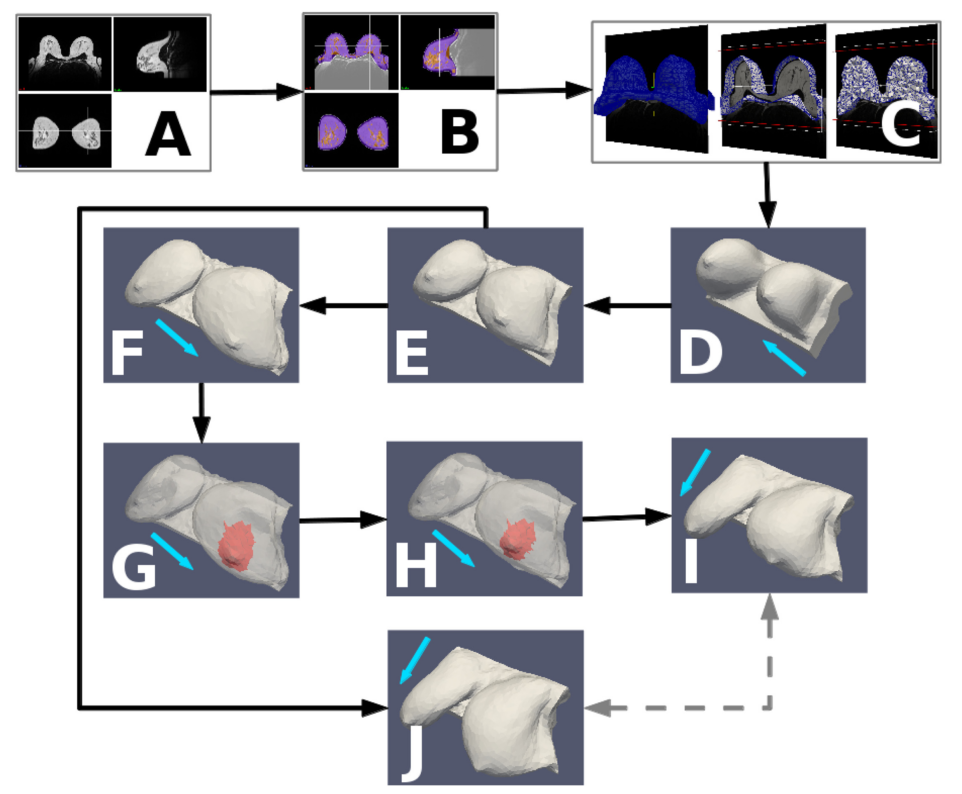
\includegraphics[width=0.85\textwidth]{oneplus}
    \caption[Example of computational process for surgical simulator]{Example of computational process for surgical simulator \cite{Vavourakis2016}}
    \label{fig:surgical_simulator}
  \end{center}
\end{figure}

\vspace{24mm}

\begin{itemize}
\item In step A, the MRI data and the computed-tomography (CT) data are acquired;
\item In step B, the data is segmented, differing the adipose and fibroglandular tissues of the breast;
\item In step C, the generation of the surface and volumetric meshes of the patient's breast is possible through the data acquisition and segmentation referred in the previous steps;
\item In step D, the models are prepared for the input of the Finite Element solver;
\item The retrieved data from MRI are represented in prone since they are stressed by the gravity force. In order to apply mechanical finite element models, the step E is required to remove the gravity effect on the model, computing the a gravity unloaded model;
\item In step F, the gravity unloaded model of the breast is converted into a supine geometry;
\item In step J, the gravity unloaded model of the breast is also used to predict the breast's geometry in upright;
\item In step G, the tumor position is identified through determining the incision lines and the outline of the excised tissue. Consequently, the elements inside the outline of excised tissue are labeled as damaged tissue;
\item Step H, performs the wound healing simulation resulting in the wound contraction and the estimation of the post-surgery breast shape;
\item Finally in step I, the effect of gravity is re-applied on the breast shape, retrieving the model in a stand up position, or upright geometry.
\end{itemize}

\vspace{12mm}

The proposed surgical simulator that estimates the wound healing and the pos-surgical shape of the breast relies on the two mathematical models described below:

\begin{itemize}
\item Wound Healing and Angiogenesis Model

This mathematical models is based on the cell density, the concentration of biochemical agents responsible for the mitosis regulation, the density of the microvascular density, the nutrient and oxygen levels and the agent that regulates vascular spouting in order to compute the changes on the breast shape during the healing process. It also takes into consideration the increase of the inflammatory response and the stimulation of the immune system.

\item Soft Tissue Biomechanics Model

Also responsible for the configuration of the breast geometry, the Soft Tissue Biomechanics model takes into account the breast tissue's mass density and the body force vector. Within this model, the stress distribution is calculated considering the passive stress of the tissues' mechanical deformations and the active stress from the tissue recovering during the wound healing process.  

\end{itemize}

\section{Existing Frameworks}\label{sec:ferramentas}

The greater portion on this field focuses on breast augmentation and plastic surgery and have originated some software able to simulate deformations on the breast tissue. Being the most known:

\begin{itemize}
\item Crisalix \footnote{\label{crisalix} \url{https://www.crisalix.com/en}}

Crisalix is a web based application based on 2D photographs with a range of implant types, sizes and surgery techniques available. Figure \ref{fig:crisalix} shows Crisalix software, that allows to simulate breast enlargement or reduction, breast lift, the application of silicone implants, implants revision, scars, breast reconstruction and fat transfer.

\begin{figure}[H]
\begin{center}
    \leavevmode
    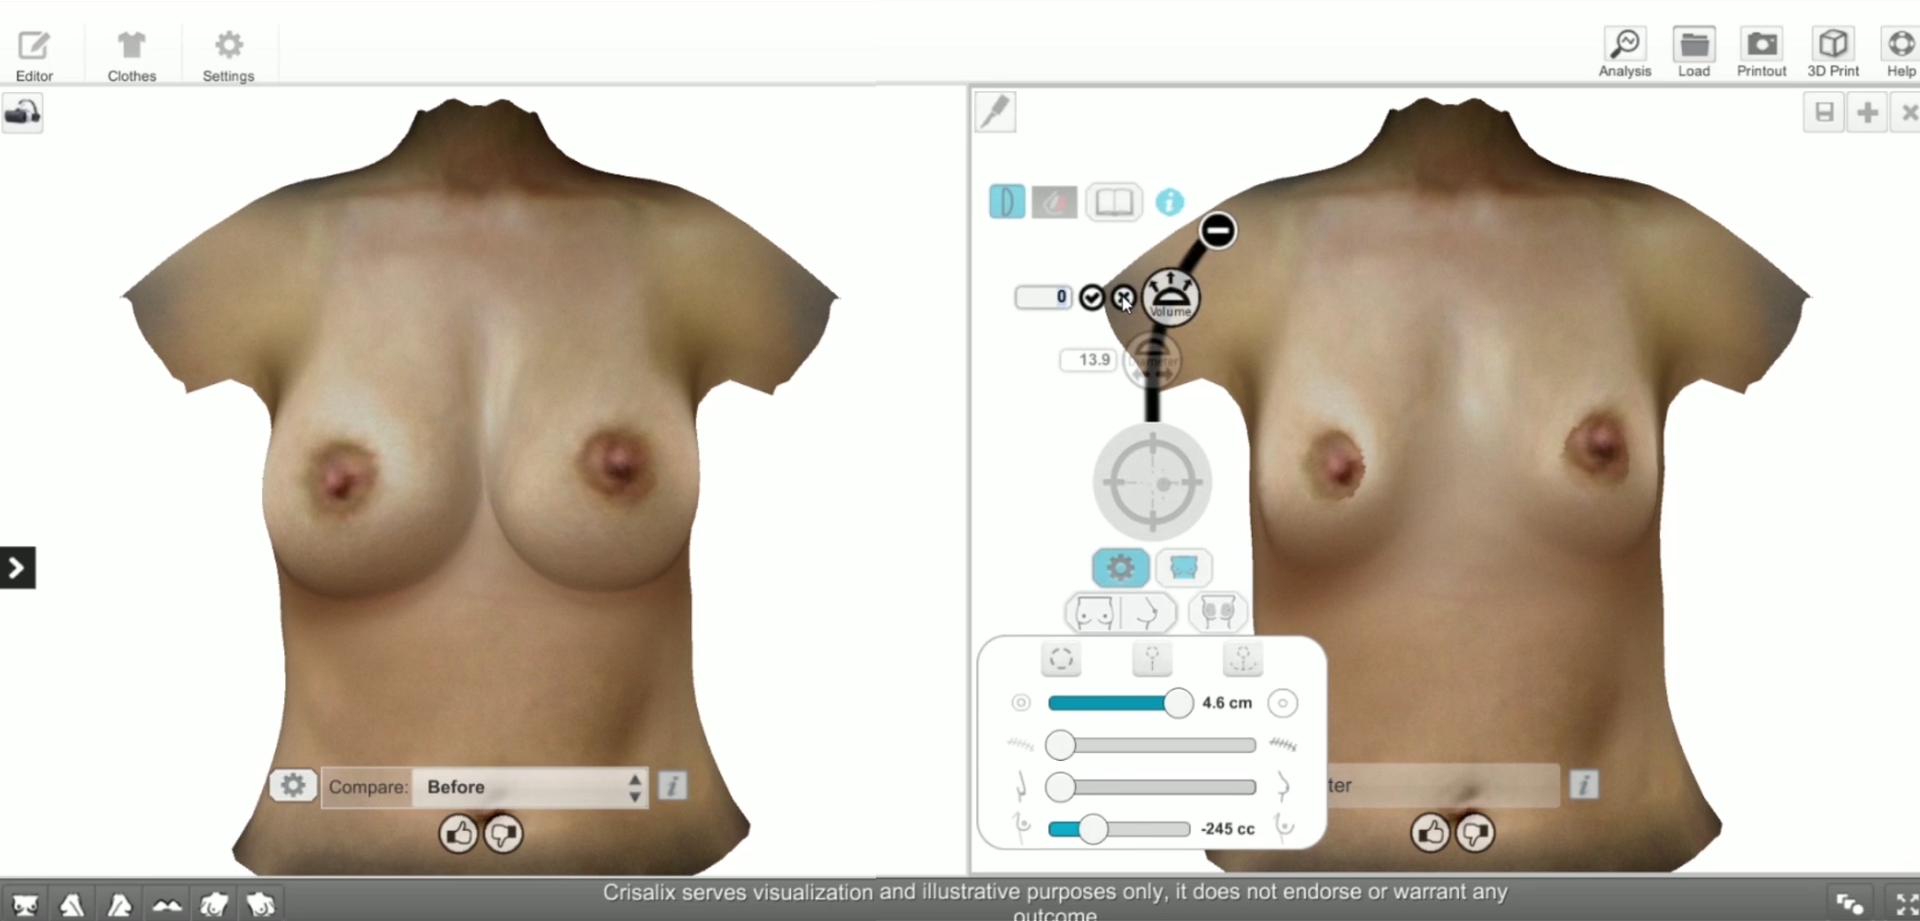
\includegraphics[width=0.5\textwidth]{crisalix}
    \caption[Crisalix interface]{Crisalix interface \textsuperscript{\ref{crisalix}}}
    \label{fig:crisalix}
  \end{center}
\end{figure}


\item Sculpt My Dream \footnote{\label{sculptmydream} \url{http://www.sculptmydream.com/}}

Sculpt My Dream is a property platform of Vectra3D, and uses six distinct cameras to reconstruct a virtual model of the patient's torso. The simulation relays on a variety of implant sizes and a list of manufacturers while is able to correct some asymmetry of the breast. Even though the good estimation and the similarity between the software simulation and the procedure, it can only be applied to plastic surgery. Figure \ref{fig:sculptmydream} shows Sculpt My Dream interface.

\begin{figure}[H]
\begin{center}
    \leavevmode
    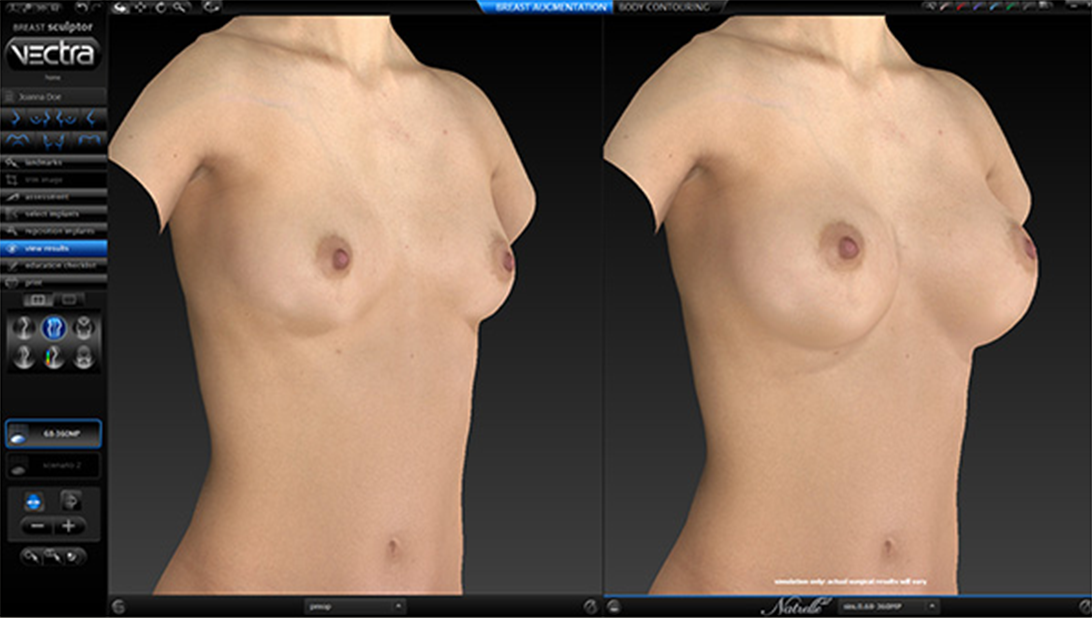
\includegraphics[width=0.45\textwidth]{sculpmydream}
    \caption[SculptMyDream interface]{Sculpt My Dream interface \textsuperscript{\ref{sculptmydream}}}
    \label{fig:sculptmydream}
  \end{center}
\end{figure}

\item Axis Three \footnote{\label{threeaxis} \url{http://www.axisthree.com/welcome}}

Axis Three uses a property scanner to capture 3D images of the patient's torso. It simulates alterations on the face or breast of the patient. In the specific case of breast simulation, it is based on the manufacturers implant, the location of the implant (beneath or above the pectoral muscle) and the tissue's elasticity. Figure \ref{fig:threeaxis} shows Axis Three interface.
 
 \begin{figure}[H]
\begin{center}
    \leavevmode
    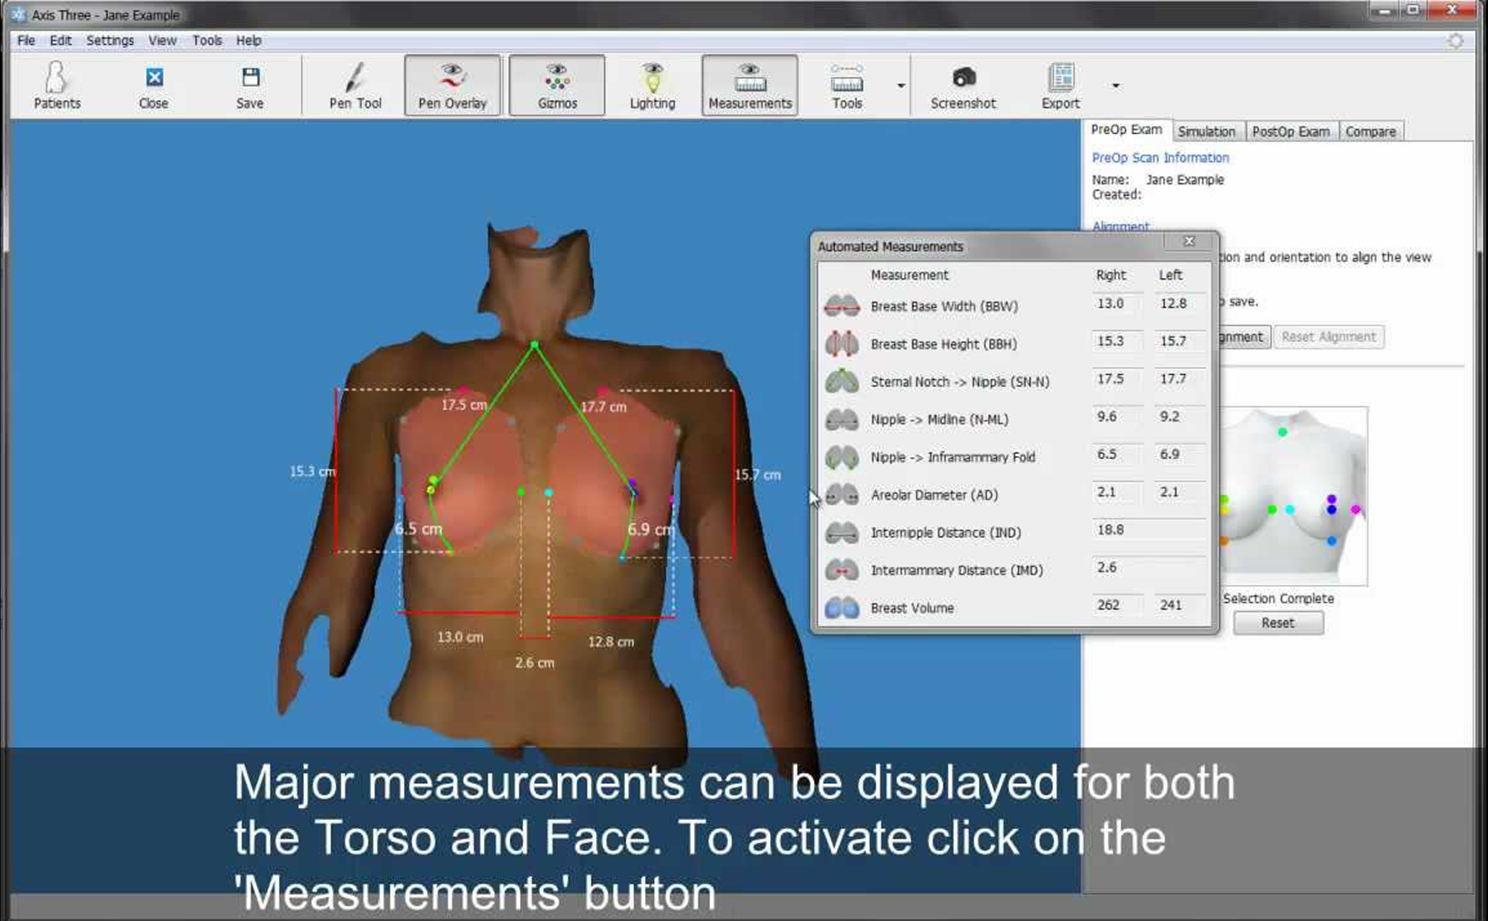
\includegraphics[width=0.45\textwidth]{threeaxis}
    \caption[Axis Three Software]{Axis Three interface \textsuperscript{\ref{threeaxis}}}
    \label{fig:threeaxis}
  \end{center}
\end{figure} 
 
\end{itemize}

In spite of the reliability of these 3D scanner, the utilization of several cameras are demandingly expensive and while it requires complicated procedure to perform 3D reconstruction of the patient's torso.

\section{Summary}

The patient's 3D models, including torso, or individual organs, have been commonly used in applications of both medical tools. In this chapter, a brief descriptions of recent methodologies have been explained as well as their medial applicastions.

Concerning the representation of humans breast, most of the studies focused on the application of the models for plastic surgery. More recently, FFD was used in order to represent the breast's shape; and FEM researched in order to simulate wound healing and transformations between different geometry configurations of the breast.

Despite of the existence of a surgical simulator, time consumption and computational power requirements of FEM makes it unviable to be used in real-time systems. Machine learning techniques will be applied in order to predict the same deformation caused by the BCS in order to overcome the problems of the FEM approach. This methodology is detailed in chapter \ref{chap:method} and its results are presented in chapter \ref{chap:results}.
